\title{Energy budget for insects}

\documentclass[12pt]{article}
\usepackage{amsmath}
\usepackage{mathabx}
\usepackage{graphics}
\usepackage[top=0.75in, bottom=0.75in, left=1in, right=1in]{geometry}
\usepackage{tabu}
\usepackage[english]{babel}
\usepackage{natbib}
\bibliographystyle{evolution}
\usepackage{rotating}
\usepackage[capitalize, sort&compress]{cleveref}
\usepackage{float}
%\newcommand{\crefrangeconjunction}{--}
%\crefname{section}{Sect.}{Sects.}
%\crefname{equation}{Eq.}{Eqs.}
%\crefformat{equation}{Eq.~#2#1#3}
%\crefrangeformat{equation}{Eqs.~#3#1#4--#5#2#6}
%\crefmultiformat{equation}{Eqs.~#2#1#3}{--#2#1#3}{, #2#1#3}{ and~#2#1#3}
 
% for comments visible in the compiled pdf
%\usepackage{color}
%\definecolor{orange}{rgb}{0.8,0.4,0}
%\newcommand{\eeg}[1]{{\em \color{orange} #1}}

% Tell latex how it can introduce linebreaks if necessary.
\hyphenation{Bar-thol-o-mew}

\begin{document}
\maketitle 

\section*{Introduction}
A principal goal in ecology is to describe and understand processes that influence species distribution.
The act of describing and explaining is not often mutually inclusive.
In some cases, things fit naturally.
Abiotic factors can easily correlate with species range.
Temperature isocline matches range limits which provides evidences of range limitiation \citep{Root1988}.
Biotic factors also plays a role in the shaping species range \citep{Krebs2000}.
Various types of interaction within and among trophic level can both expand or contract species distribution.
In the most general case, it is not evident which factor is most important.
Sometimes, several factors are correlated and disentangling the relative effect of these  factors is a difficult task.

A surrogate approach is to flip the question around; choose a factor and see how it affects the performance of the species, given everything else is equal.
Temperature is one abiotic that has been investigated in depth.
Controlled experiments have been conducted to see how species responds to gradient of temperature.
It is often complicated to directly measure fitness and instead rely on proximate variables (performance) such as locomotion, growth rate, assimilation, fecundity rate \citep[][and reference therein]{Angilletta2009}.
A classical results is that thermal performance is non monotonic and is skewed to the left meaning that the optimal temperature (peak of the curve) is closer to the critical maximum temperature for positive performance than the minimum temperature. 
Whereas the approach looking the marginal effect of one factor is difficult of empirical study (it can be logistically difficult to keep everything else equal), it is the basic philosophy behind a theoretical approach.

Theoretical works have investigated the role of temperature in shaping performance especially in growth \citep{}. % Kozlowski, vanderhave  
Recently theoretical work has underpinned mechanisms that look directly at fitness \citep{Amarasekare2012}.
The model  breaks down thermal performance (intrinsic growth rate)  into three components: development, fecundity, and mortality.
The functional shapes of each of these components thus determines the basic properties of the curve.
Not only, the left-skewed is recovered but the model provides an explanation of why it is left-skewed--because of how the three component behaves. 
A different model that dig deep into physiological principles is called Dynamic Energy Budget (DEB) \citep{Kooijman2009}.
The model focuses on how (food) energy is assimilated and then allocated to different needs such as growth, metabolic cost (maintenance), reproduction \citep{Kooijman2009}.
When species data are available, these models are excellent in reproducing the pattern. 

Such model framework helps us understand that performance curves and how they differs  among individuals, but it does not provide a framework for understanding the intrinsic causes of those differences.
One variable that might underlie those differences is body size.
Empirical data have shown that body size is often associated with temperature.  
For instance, individual grows larger under colder thermal regime \citep{Van1996}.
Metabolic theory of ecology links with one equation body size and temperature \citep{Brown2004}.
There is even a pattern at global scale, the Bergman's rule which states that body size tends to increase with decreasing temperature \citep{Bergman1847}. 
Theoretical study tends to look at the role of body size without taking into account explicitly temperature.
The question thus remains, given everything else is equal how does thermal performance curve changes with body size?

A lot of ecological process are influenced by body size \citep{Peters1986}.
Of the most well known is metabolic rate is known to scale with body size by following a power law.
Many of empirical and theoretical studies have attempted to get the correct relationship.
An important process that is often overlooked is the role of behavioral thermoregulation for performance. 
For cold blooded animal, thermoregulation is an important part of the daily activity.
In warm environment, species thermoregulate to avoid overheating.
For instance, some insects avoid overheating during flight by dissipating excess heat from the thorax to the abdomen \citep{Verdu2012}.
In cold environment, some individuals also regulates avoid losing heat.
In a cold environment, some insects have the opposite strategy that insulate the thorax from the rest of the body to keep heat \citep{Verdu2012}.
Muscle needs to be at certain temperature to function properly thus when the environment is below that temperature, an individual needs to do warm-up. 
For cold blooded animal, the general strategy is to bask under the sun and absorb the heat.
In this case, body size have a direct influence as it mediates heat absorption (conductance) and in general exchange via surface-area to body size ratio.
Buckley included warm-up process of a species of lizard but the role of such process in shaping thermal performance in general level has not been explored. 

In this work we build a theoretical model to investigate how thermal performance varies with body size for cold blooded animals. 
Our approach is to look at the effects of three processes: physiological processes based on metabolism, ecological factor which depends on resource availability and foraging, and thermodynamical factor, thermoregulation processes.
The philosophy of the model is the same as energy budget model, here we define performance as difference between total energetic gain and energetic cost.
We narrow our taxonomic scope to insect, more precisely to adult insect with deterministic body size and income breeder. 
In general, we found the metabolism plays a secondary role in shaping thermal performance.
Instead, resource availability and allometric scaling of foraging are key in defining the upper thermal limit whereas thermoregulation ability of warm-up sets the lower thermal limit.

\section*{Model Description}

%\label{model description} \cref seems not to work when section*
% E: The proper solution is to use \section{} instead of \section*{}, and to use \setcounter{secnumdepth}{0} in the preamble to suppress numbering.

The model investigates the daily performance of an adult insect with fixed body size.
We define performance as net energy gain, which is the difference between energetic gain and loss during the day.
The energetic gain is the amount of energy acquired during solitary foraging, whereas the energetic loss is the sum of metabolic costs incurred while resting and during foraging activity.
The model contains a thermoregulation phase that precedes activity.
It thus applies to insects that must complete warm-up because muscles are only operational when they are above a certain temperature.
The model is built by describing relationships among several variables (\crefp{fig1}a).
% E: Side note: \crefp{} is for references inside parentheses; AmNat abbreviates them.
First, we describe the external properties of the environment.
Second, we use empirically derived relationships to model the rate of energetic loss and gain as a function of body size and temperature.
Third, we use thermodynamic principles to describe changes in body temperature during warm-up.
Finally, we integrate these components to define net energy gain.
We then further justify the functional forms and parameters employed by our model.

\subsection*{Environment}

We consider three properties of the environment: the temperature, the intensity of solar radiation, and the amount of available resource.
We define environmental temperature $T_e$ as the temperature felt by the individual while inactive.
%We implicitly assume that environmental temperature takes into account other factors such as humidity and so on.
Because insects are small, we assume that environmental temperature does not depend on body size. % E: How would it for large individuals?  Self-shading? T: Dinosaurs are thought to be almost homeotherm because the loss of heat is so low.
Our model derivation here does not account for temperature variation during the day, but we show in the Supplementary Figures that daily temperature changes do not affect the qualitative results.

We assume that at any given time of the day, the intensity of solar radiation is $S_R = S_0 \cos(\psi)$,
where $\psi$ is the zenith angle and $S_0 = 1361 \, \rm{W m}^{-2}$ is the maximum solar radiation at noon.
Solar radiation is needed to generate heat during the warm-up phase of the model.
See the Appendix and \citet{Campbell2012} for more details on how $\psi$ depends on latitude and the day of the year as well as how we obtained the time of sunrise.

We denote by $R$ the daily quantity of resource available.
The energy density per unit of resource mass is $\rho$.
Poor environments in terms of resource can thus be obtained by low quantity $R$ or low quality $\rho$.

\subsection*{Energetic cost}

\subsubsection*{Resting metabolic rate}

Following \citet{Brown2004}, we assume that resting metabolic rate increases with body size and temperature such that
\begin{equation} \label{eq:eb}
	e_b(z, t) = a_1 z^{b_1} \exp \left(\frac{-E}{k (T_b(t)+ 273.15)}\right),
\end{equation}
where $z$ is body mass, $T_b(t)$ is the body temperature at time $t$ in Celsius, $E$ and $k$ are respectively the activation energy and the Boltzman constant (this is the Arrhenius equation), and $a_1$ and $b_1$ are constants which we call respectively the coefficient and exponent.
At rest, the body temperature of the individual matches that of the environment \citep[e.g.,][]{Bartholomew1978} so that $T_b(t)$ in \cref{eq:eb} can be replaced by $T_e(t)$.
% T: I realize here that temperature in the beehive can differ from T_e!!! I would say it does not matter much but...if one wants to be picky???
% E: Oh, right!  So then you warm up in one environment and go be active in another... too much complication for no clear gain, I think.

\subsubsection*{Active metabolic rate}

For simplicity and because it is poorly characterized empirically, we assume that the functional form of the active metabolic rate is the same as that of the resting metabolic rate, i.e.,
\begin{equation} \label{eq:ea}
	e_a(z,t) = a_2 z^{b_2}  \exp \left(\frac{-E}{k (\max[T_w(z_{th}), T_e(t)]+ 273.15)} \right),
\end{equation}
where $T_w$ is the minimum thoracic temperature that would permit foraging.
The warm-up phase (see section Warm-up below) determines whether an individual is able to warm up and eventually forage. % should \cref with section but it did not work, later...
Large-bodied individuals often have higher temperature during activity, so we allow $T_w$ to depend on $z_{th}$, as in \citet{Bartholomew1977a}:
\begin{equation} \label{eq:Tw}
	T_w(z_{th}) = c_0+ c_1 z_{th}.
\end{equation}
Here, $z_{th}$ is the mass of the thorax, and $c_0$ and $c_1$ are two free parameters.
Thus, unlike resting metabolic rate (\crefp{eq:eb}), the effect of temperature on active metabolic rate depends on body size.
The use of the function `maximum' ($\max$) is a rough approximation such that when the environmental temperature is too high, there is an additional cost of foraging, such as the additional energy used to avoid overheating.
To ensure that the cost of activity exceeds that of resting, we assume that the parameters of the active metabolic rate are not less than the parameters of the resting metabolic rate, i.e., $a_2 \geq a_1$ and $b_2 \geq b_1$. % E: either "greater than" and ">" or "greater or equal to/not less than" and "\geq"

\subsection*{Energetic gain: foraging}

We define foraging rate $g(z)$ as the average amount of resource an individual collects per unit of time.
Here, given that absolute metabolic cost increases with body size (\crefp{eq:ea}), we assume that foraging rate also increases with body size, and for simplicity, we assume a power law,
\begin{equation} \label{eq:g}
	g(z) = a_3 z^{b_3}.
\end{equation}
This equation pools together different activities such as searching for and handling the resource.
We will not assume any particular value for $b_3$, and our results explore its role in shaping thermal performance.
If small individuals are more agile, \cref{eq:g} takes a concave shape (\crefp{fig1}b).
Alternatively, if large individuals have better searching ability (e.g., they find more distant resources), \cref{eq:g} takes a convex shape.
Finally, the rate of energy gain includes both foraging rate and resource quality:
\begin{equation} \label{eq:eg}
	e_g(z) = g(z) \rho = a_3 z^{b_3} \rho.
\end{equation}

\subsection*{Warm-up}

As we mentioned earlier, when environmental temperature is low, an individual needs to reach sufficient internal temperature to be active for foraging.
In general, warm-up behavior would include the when, where, and how of warming up.
Here, however, we focus on whether or not warm-up can be completed, and if so, the duration of warm-up.
Furthermore, insects do not need to warm up the entire body, only the thorax where most of the muscles are \citep{Kammer1974, Heinrich1975, Bartholomew1978, Verdu2012}.
Therefore, we track the temperature of the thorax, $T_w$ (\crefp{eq:Tw}), and so focus on thoracic mass, $z_{th}$, rather than body mass.

The most common strategy for warming up is to absorb solar radiation.
Heat is transfered to the thorax from the surface of the body by passive conductance \citep{Bakken1976}.
A second strategy is to endogenously generate heat by contracting muscles against each other, similar to shivering \citep[e.g.,][]{Kammer1974}.
We assume that the frequency of contraction increases linearly with thoracic temperature: $f(T_{th}) = a_w T_{th}$ for $T_{th} > 0$ and 0 otherwise.
We loosely use the term ``endotherm'' for insects that have the ability to generate heat endogenously during warm-up ($a_w > 0$), and ``ectotherm'' for insects that do not generate heat ($a_w = 0$).

Coupled differential equations  track changes in the thoracic temperature and non-thoracic temperature (i.e., the rest of the body) during warm up.
For geometrical simplicity, we assume that the body is half of a sphere and the thorax constitutes half of the body.
The surface of the thorax and the non-thorax can be easily calculated given the mass and the density of the insect (see Appendix).

Change in thoracic temperature, $T_{th}$, is based on heat exchange between the thorax and the non-thorax.
We have
\begin{equation} \label{eq:dTh}
	\frac{dT_{th}}{dt} = \frac{1}{s z_{th}} \left[ z_{th} e f(T_{th}) +  A_{th} K_1(T_r - T_{th}) \right],
\end{equation}
where $s$ is the specific heat capacity, $e$ is the calories generated per contraction and per gram of muscle \citep{Kammer1974}, $A_{th}$ is the total surface of the thorax, and $K_1$ is the conductance between the thorax and the non-thorax.

Change in the  non-thorax temperature ($T_r$; the subscript $r$ is to remind us it is the rest of the body) is based on thermal exchange between the surface of the individual and the external environment.
We have
\begin{equation} \label{eq:dTn}
	%\begin{split}
		\frac{dT_r}{dt} =  \frac{1}{s z_{r}} \left[ - A_{th} K_1(T_r - T_{th})  \right]
			+ \frac{1}{s z_{r}} \left( A_r \left[ - c_p K_2 h(T_r -T_e, V)- \sigma \varepsilon T_r^4 + \sigma \varepsilon T_e^4  + r_3 S_R  \right] \right),
%\end{split}
\end{equation}
where $\varepsilon = 0.935$ is the emissivity of a gray body, $u$ is wind speed, $V$ is the volume of the insect, and $A_r$ is the surface area of the non-thorax (simply the surface of the whole body).
We consider two forms of convection here, with $ h(T_r -T_e, V) = (T_r- T_e)^{1.25} (1/V)^{1/12 }$ for free convection (no wind) and $ h(T_r -T_e, V) =  1.4 \times 0.135 \sqrt{u/V^{1/3}} (T_r- T_e) $ for laminar convection \citep{Campbell2012}.
%
The conductance $K_1$ is defined above, and $c_p$ is the specific heat capacity of the air.
The constant $K_2$ controls convection between the body and the air \citep{Campbell2012}.

The last term of \cref{eq:dTn}  is an approximation of more the detailed equation in \citet{Campbell2012}.
Here, we ignore view factors, reflected radiation and so on, and pool every source of radiation into $ \sigma \varepsilon T_e^4$ and $S_R$.
The parameter $r_3$ is used to scale and summarize the quantity of absorbed solar radiation.

We solve the ODE system (\crefp{eq:dTh,eq:dTn}) numerically using the function NDSolve in \nocite{Mathematica10} Mathematica.
By solving the equations through time, we can find if the minimum temperature  required for activity ($T_w$) is reached. % E: Be prepared to submit your Mathematica notebook as a supplemental file (as .nb and .pdf).
If it is, we can also solve for the duration of the warm-up $\tau_w$ from $T_{th}(\tau_w) = T_w$.

\subsection*{Net energy budget}

We now integrate all the components above to calculate the energy budget during a 24-hour period.
Daily activity consists of resting, warming up, and foraging activity.
We assume activity occurs in one block of time and thus require only one warm-up phase. % E: as opposed to "continuous activity" meaning that it never ends
We use $t$ to denote the time of the day and $\tau$ for duration.
% We start the calculation at sunrise, $t = 0$ and end at $t = 24.$
Total foraging time, $\tau_f$, can be fixed, or it can be a function of resource availability $R$, with $\tau_f = R/g(z)$.
(We always assume that an individual can gather at most 50 times its body mass.)
If warm-up cannot be completed, foraging does not occur and $\tau_f = 0$.
If warm-up is completed, we penalize the individual by subtracting the duration of warm-up $\tau_w$ from the total foraging time $\tau_f$.
Referring to \cref{eq:eg}, the total daily energetic gain is given by
\begin{equation} \label{eq:Eg}
	E_g(z,\tau_f - \tau_w) = (\tau_f - \tau_w) e_g(z).
\end{equation}
If we assume that warm-up starts at $t_i$ the total daily energetic cost is
\begin{equation} \label{eq:Ed}
	E_d(z, \tau_f) = \int_0^{t_i} e_b(z, t) dt + \int_{t_i + \tau_w}^{t_i + \tau_f } e_a(z,t) dt + \int_{t_i+\tau_f}^{24} e_b(z, t) dt,
    % E: I presume the t subscript on E stood for "total", but it is a bit confusing with t also meaning time.  So I changed to E_d (for "daily") here and in the Appendix, or pick something else.
\end{equation}
where $e_b$ is defined in \cref{eq:eb}  and $e_a$ in \cref{eq:ea}.
The first and the last term on the right hand side calculate the total energetic cost when the individual is at rest from $t = 0$ to $t = t_i$ (before foraging) and from $t = t_i + \tau_f$ to $t = 24$ (after foraging).
The middle term calculates the total energetic cost of foraging from $t = t_i + \tau_w$ to $t = t_i + \tau_f$.
% E: Consider dropping the "t =" in the previous sentences.  Or add it in the next sentence.
Our calculations show that the energetic cost while warming up from $t_i$ to $t_i + \tau_w$ is negligible, for both endotherms (actively shivering) and ectotherms (passively basking).
We thus omit it from \cref{eq:Ed}, in accord with empirical findings \citep{Heinrich1975}.

Daily net energy gain is obtained from the difference between energy gain from foraging (\crefp{eq:Eg}) and total energy expended (\crefp{eq:Ed}), i.e.,
\[
	E_n(z, \tau_f) = E_g(z,\tau_f- \tau_w) - E_d(z, \tau_f).
\]

\subsection*{Power law and parameter justifications}

Our model assumes that the relationships between body size, metabolic rate, and foraging rate are represented by power laws.
A general pattern is that resting metabolic rate scales with body size with an exponent $b_1 = 0.75$ (\crefp{eq:eb}), which has been reported from unicellular organisms to mammals \citep{Kleiber1947, Peters1986,Gillooly2001,Brown2004}.
Although there is a debate about the actual values \citep[e.g.,][]{Isaac2010}, we adopt that value to diminish the number of free parameters, allowing us to explore the values of other exponents that are less-well established.

The power law relationship for active metabolic rate has much less empirical grounding, with few studies measuring it for a range of body sizes.
A notable exception is work by \citet{Bartholomew1978}, who found a power law with exponent $b_2 = 1.17$.
More studied is metabolic scope, which is the ratio of maximum active metabolic rate to resting metabolic rate.
Many factors such as foraging mode (flying vs. walking) yeild a substantial variation in metabolic scope.
Oxygen consumption during activity can range from 2 to 100 times that of resting \citep{Bartholomew1978, Bartholomew1981, Bartholomew1985, Chown2004, Niitepold2010} although a typical value would be between 10 to 40-fold increase \citep{Bartholomew1981, Niitepold2010}. %Bartholomew and Lighton 1985 for 2 fold.

Recent studies of the rate of energetic gain have recovered a power law relationship \citep{Pawar2012, Maino2015}.
There seems to be no single exponent $b_3$.
For instance, the exponent can depend on the dimension of the search space, with a value of 0.85 in two dimensions or 1.06 in three dimensions \citep{Pawar2012}.
Body size can further influence other processes.
For instance, walking speed  can scale with a power 0.29 \citep{Peters1986}, or dominance competition exerted by larger individual can yield an exponent greater than one.
Our goal, however, is not to assert the homogeneity of these values but instead to explore the consequences of their heterogeneities.

The effect of temperature could be modeled by multiplying the body mass scaling metabolic rate with a factor $Q_{10}$, which denotes the change in metabolic rate with a $10^ {\circ} \rm{C}$ increase in the body temperature \citep{Precht1973}.
We however opted for the Arrhenius equation (\crefp{eq:eb}) used by \citet{Brown2004} because it reduces the number of free parameters, and it also approximates the temperature effect for $Q_{10} = 2.45$.

The model parameter values will of course vary across organisms and environments.
For instance, the coefficient of resting metabolic rate or exponent of foraging rate might be different for ants and dung beetles.
Our goal is not to predict specific energetic values, however, but to explore the effects of these general processes on thermal performance curves.
Our conclusions are thus best interpreted as applying across individuals within species, or across species that are closely related.
\cref{table:table1} summarizes the range of parameter values considered in our analyses.

% E: To print the table at the end of the manuscript, I moved it to a separate file.

\section*{Results}
The results are partitioned into 3 parts.
Many things go into performance. We  single out the effects here.
 Ask, when can performance peak at intermediate body size.

- Physiological and ecological processes.
When resource or time is limiting.

Fig 1 shows how net gain changes as function of body size

 Case 1: when resources are low, the gain cannot compensate for large and thus net gain decreases with body size. 
 This effect vanishes as resource increases, net energy gain increases as function of body mass.
 What it is interesting here is that exponent of foraging rate, or metabolism, and metabolic scope interferes only quantitatively. 
 
 Case 2: we now look at the role of temperature.
 Temperature increases the metabolic cost.
 Foraging is constant here but we vary the cost being active ($b_2 = 1.25, a_2 = 40$).
 Even if resources are unlimited.
 As temperature increases, it becomes more costly for large given that $b_3$ is low. 
 The ratio plays a role here.
 As a contrast, when b3 is high, only large can persist. 

 It is worth to mention that foraging time differs here and this for low b3, it takes longer for large to get 50 times the resources and thus even higher active metabolic rate   
 
 Fig 2 shows when time is limiting
 In the same scenario as above, large is always advantageous when b3 is high enough.
 When b3 is low the same hump pattern occurs.
This only happens at specific situation.
First, net energy can should increases and then decrease after certain threshold (thus looking at the derivatives)
Second, net energy should also be positive.
These conditions are fulfilled when: 

 There are two things: the $b_3$ as we have seen before but also, resource quality matters.
 Sound too restrictive. 
 

We explored the influences of two internal parameters: $b_3$ (\cref{eq:eg}) which scales the effect of body size on resource allocation and conductance $K_1$ and $K_2$ which defines the passive loss of heat during warm-up, convection, and two environmental variables: environmental temperature $T_e$ and the amount of resource available $R$.

Our main goal is to understand the role of different processes in shaping the energy budget of a species given its body mass.

% E: Good strategy to give basics of model behavior first, and then put it together for the more complicated niche questions!

\subsection*{Role of foraging and cost of metabolism}
We look at the cases that can limit the amount of resources that an individual can acquire.
The first case is when the amount of resource available is limited (\cref{fig1}).
When there is not enough resource, the high energetic demand of large individual due to higher metabolic rate cannot be compensated.
As a consequence, as net energy gain decreases as function of body size (\cref{fig1}ab).
When resources are not limiting, net energy gain increases with body size.
More importantly, the foraging exponent $b_3$ only changes the pattern qualititatively.

The situation may be different when temperature is varied.
By increasing the metabolic scope (high cost of activity), large individual shows two contrasting responses.
When foraging exponent is low ($b_3 = 0.5$ ), performance is again maximized at intermediate value even if resources are not limiting (\cref{fig1}d vs. \cref{fig1}e).
Increasing temperature puts more pressure on large individuals as the metabolic cost is higher.
When foraging exponent is high $b_3 = 1.25$, only large individual can persist (\cref{fig1}f).

The second case is when the time available for foraging is limited (\cref{fig2}).
In general, net energy gain increases as function of body size.
However, like in the previous case, when $b_3$ is low, maximum net energy gain is attained at intermediate body size (dashed line, \cref{fig2}a). 
The analytical result shows that net energy gain only peaks when two conditions  are met.
First, $b_3 < b_1 = b_2$ (the equality is by assumption and to reduce the number of free parameter).
% E: so really, the condition is that b_3 is the smallest? 
% T: yes
Second, resource quality $\rho$ is within a certain range represented by shades in \cref{fig2}a.
\cref{fig2}b shows for two different temperatures (red = warm, blue = cold) the required values of the resource quality $\rho$ so that net energy gain peaks at intermediate value of body mass.
\cref{fig2}c shows how net energy gain changes as function of body mass for the resource quality shown in \cref{fig2}b.
These conditions are quite restrictive and looks unlikely in real system.
% E: This is a great example of why it was worth constructing a math model, rather than just intuitive arguments!

In a more technical term, the range of the $\rho$ allowing intermediate optimal body mass is 
\begin{equation}\label{C1}
	\widetilde{E_n} < \rho < \widetilde{dE_n}.
\end{equation}
where,
\begin{flalign*}
\widetilde{E_n} &= \theta_1 + \theta_2, \\
\widetilde{dE_n} &= \frac{b_2}{b_3} \theta_1  +  \frac{b_1}{b_3} \theta_2.
\end{flalign*}
and $$\theta_1 = \frac{a_2}{a_3}  z^{b_2 - b_3}  e^{-E/[k (max(T_w(z_{th}),T_e(t))+ 273.15)]}$$ and $$\theta_2 =  \frac{a_1}{a_3} z^{b_1- b_3}  e^{-E/[k (T_e(t)+ 273.15)]} (\frac{24}{t_f} -1).$$

The difference between  $\widetilde{E_n}$ and  $\widetilde{d E_n}$ is that in  $\widetilde{dE_n}$, each term of  $\widetilde{E_n}$   is weighted by $\frac{b_2}{b_3}$ and $\frac{b_1}{b_3}$.
Thus, a necessary condition for optimal mass to be intermediate (\cref{C1}) is that the weights are larger than 1 i.e.  $b_3 < b_1$ ($b_2 \geq b_1$ is always true). 
As temperature increases, the term with the product $\frac{b_1}{b_3}$ becomes larger thus increasing the range of values where \cref{C1} is true (\cref{fig2}a).

Note  that the bandwidth is broader in warm than in cold environment.
This is because in warm environment , the $\theta$s are larger arithmetically and not geometrically.
It is easier to use example. 
For simplicity, if $\theta_1 = \theta_2 = 1 (10)$ small (or large) and $b_1 =b_2 = 0.75, b_3 = 0.5$.
For small, the range is $\theta_1 + \theta_2 = 2 < \rho <  0.75/ 0.5 \theta_1 +  0.75/0.5 \theta_2 = 3.$  
For large, the range is $\theta_1 + \theta_2 = 20 < \rho <  0.75/ 0.5 \theta_1 +  0.75/0.5 \theta_2 =  30.$  


\subsection*{Role of warm-up.}
\subsubsection*{Minimum conditions}
Successful warm-up is a necessary condition before foraging. 
Under perfect conditions where solar radiation is not limiting and forced convection from wind is absent , any individual can absorb use that energy to warm-up.
We explore here cases where solar radiation is limiting and wind increasing convection between the surface of the individual and the external environment.

Three different ways the minimum temperature required to complete warm-up vary as a function of body mass (\cref{fig3}).
First, the minimum temperature for warm-up increases with body mass because small individual absorbs more heat--higher surface area-to-body ratio (\cref{fig3}a).
This pattern only occurs when the individual relies only solar radiation to warm-up (ectotherm) and there is only free convection (no wind).
Second, the minimum temperature for warm-up is lowest at intermediate body size (\cref{fig3}b). 
This happens because there is now more convection due to wind. 
Small individuals are  penalized as convection increases (see \cref{eq:dTr2}).
Third, minimum temperature decreases with body size (\cref{fig3}c).
It occurs when individuals are capable of producing heat endogenously (endotherm).
In this case, the role of surface area-to-body ratio is reversed as the heat generated in the thorax dissipates less with large individuals.
% E: I repeat my comment above: This is a great example of why it was worth constructing a math model, rather than just intuitive arguments!

\subsubsection*{Duration of warm-up.}
Another aspect of warm-up is the time it takes to complete it.
As expected, duration of warm-up decreases as this intensity of solar radiation increases (it peaks at noon) (\cref{fig4}).
The decrease is not linear, warm-up time decreases abruptly and then level off few hours after sunrise (\cref{fig4}a).
For endothermic individual, the same pattern occurs although it is less abrupt compared to ectothermic individuals (\cref{fig4}b) .
For ecothermic individuals, the duration of warm-up increases with body mass (\cref{fig4}a).
For endothermic, it is not necessarily true because the smallest individual can lose too much of the heat it generates to the environment via conductance (\cref{fig4}b).

Conductance between the thorax and the rest-of-the-body plays an important role for the warm-up process and, as expected, has opposing roles for ecotherm and endotherm.
For endotherm, \cref{fig4}c shows how different values for the conductance are favored at different parts of the day.
If warm-up is initiated early in the day where solar radiation is weak, low conductance is better (thick line \cref{fig4}c).
As the intensity of solar radiation increases, it becomes a dominant source of energy and transferring that energy to the thorax is better achieved with high conductance (dashed line \cref{fig4}c).

\subsection*{Niche as a sum of physiological and behavioral processes.}
Now we integrate those components together to see how they shape the net energy gain as function of temperature. 
We also include performance when daily temperature changes. 
In that case and for simplicity, we assume that temperature increases linearly from sunrise to mid-afternoon and then decreases again (see appendix). 
There is no temperature at the previous and next sunrise.

\cref{fig5}a shows a default scenario with intermediate resource abundance.
For a range of daily temperature, net energy gain is highest at intermediate body size, large is not optimal for the same reason as in \cref{fig1}.
As resource abundance decreases, net energy gain decreases for larger individuals (solid lines \cref{fig5}b).
This makes small individual (relatively) more competitive and actually perform better at high temperature.
Also note that the upper limit of the `niche' is contracted to lower temperature (\cref{fig5}b), simply because the amount of resource available does not compensate the high energetic cost.

When we integrate warm-up processes, which is important when temperature is cold, large individual is also more affected.
Because it takes too much time to warm-up (\cref{fig4}bc) whether one is endothermic or ectothermic.
We assumed here that time spend during warm-up is subtracted in the total time available for foraging.
In short, warm-up contracts the lower part part of the niche.
Supplementary material contains more detailed results where warm-up cannot be completed so that the lower limit will be dictated by the patterns in \cref{fig3}.
...
% E: discuss endo vs ecto?

Finally, we look at variation in daily temperature.
Instead of having constant daily temperature, we assumed that increases throughout the day.
This increases in temperature further affects the largest individual (thick line in\cref{fig5}d).
The first reason is depicted in \cref{fig1}def where temperature increases disproportionately increases the energetic demand of large individuals even if resources are unlimited.
The decline of large individual will be unavoidable when resources are limiting (\cref{fig1}ab and \cref{fig5}d).




\section*{Discussion}
Know the fundamental niche, reaction norm, proxy for fitness, performance curve.
Many models
Niche Mapper
Buckley model
Brown

General model
Complexity for parameterization

Body size and temperature

Endotherm and nocturnal.


Behavior: Warm-up, timing of dial and seasonal activity (supported by Kearney)
Limited or increased foraging time. 

Importance of foraging.
Resource availabilty. 
Kearney vegetation cover.

Non linearity in evolutionary model

Influence of fluctuating temperature

Missing:
humidity
conversion to offspring
mortality




\section*{Figure captions}
\begin{figure}[H]
\begin{center}
%\scalebox{1.5}{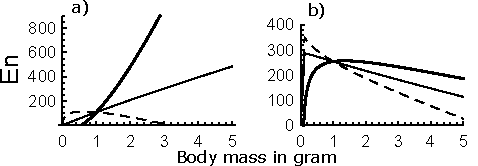
\includegraphics{Fig1}}
\caption{
	A caricature of how the exponent influences the concavity (convexity) of the power in the power law relationship.
	The black and gray lines represent foraging and active metabolic rates.
	The exponent of the metabolic rate is a bit lower to visualize to assure that the gain is more than the cost most of the time.
}
\label{fig1}
\end{center}
\end{figure}
\vspace{-1.5cm}
%
\begin{figure}[H]
\begin{center}
%\scalebox{1.5}{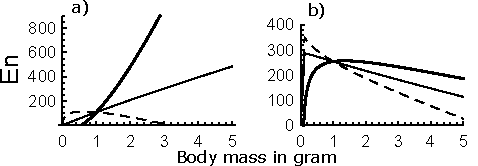
\includegraphics{Fig1}}
\caption{
	No warm-up and resource is limiting.
	Daily net energy gain  $E_n$ as function body mass $z$ for different value of foraging exponent $b_3 = 0.5, 0.8, 1.25$, dashed, thin, thick lines respectively.
	The upper panels depict different resource availabilities at $15 ^{\circ} \rm{C}$. 
	Low resource = 2.5, intermediate resource= 20, unlimited resource means an individual can collect 50 times its body mass, $b_2 = 0.75, a_2 = 20 a_1$. 
	The lower panels depict the influence of temperature when resources are unlimited and high active metabolic rate $a_2 = 40 a_1, b_2  = 1.25$.
	Low, mild, and high temperature = $5, 15, 25^{\circ} \rm{C}$.
	Fixed parameter values: $b_1 = 0.75, \rho = 16$.
}
\label{fig2}
\end{center}
\end{figure}
\vspace{-1.5cm}
%
\begin{figure}[H]
\begin{center}
%\scalebox{1.5}{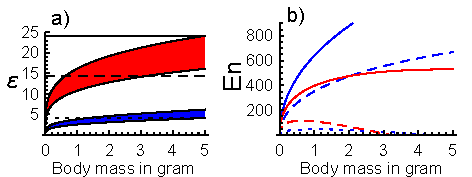
\includegraphics{Fig2}}
\caption{
	No warm-up and foraging time is limited to 0.5 hour.
	a) Daily net energy gain  $E_n$ as function body mass $z$ for different value of foraging exponent $b_3 = 0.5, 0.8, 1.25$, dashed,think, thick lines respectively  at $15 ^{\circ} \rm{C}$.
	b) $E_n$ is maximized at intermediate value of $z$  when shaded regions and resource quality $\rho$ intersect (i.e., \cref{C1} is satisfied).
	Warm ($35^{\circ} \rm{C}$) and cold (15$^{\circ} \rm{C}$) environmental temperatures are denoted by red and cyan, respectively.
	The upper (lower) limit of the shade region is $\widetilde{dE_n}$ ($\widetilde{E_n}$).  
	c) Various shapes of $E_n$ based on b).
	In b) and c), $\rho = 13, 60, 100$ dashed, thin, and thick, respectively.
	Fixed parameter values: $b_1 = b_2 = 0.75, a_2 = 5 a_1, $.
}
\label{fig3}
\end{center}
\end{figure}
\vspace{-1.5cm}
%
\begin{figure}[H]
\begin{center}
%\scalebox{1.5}{\includegraphics{Fig3}}
\caption{
	Lowest temperature required for the completion of warm-up as a function of body mass.
	The individual is given a maximum of 6 hours to complete warm-up.
	The thorax is half of the total body mass.
	To focus on the effect of solar radiation, daily temperature is constant.
	Solar radiation increases linearly from 0 to 0.25 of the maximum value $S_0$ during a period of 6 hours. 
	a) conductance is low (0.1 $\times$ the default value).
	b) conductance is default, wind speed  = 0.1m/s.
	c) For endotherm with free convection $a_w = 1.25$. 
	Fixed parameter values: default conductance $K_1 = 0.05 c_p, r_3 = 0.5$.
	Remaining parameters are in table 1.
}% Add parameter values later
\label{fig4}
\end{center}
\end{figure}
\vspace{-1.5cm}
%
\begin{figure}[H]
\begin{center}
%\scalebox{1.5}{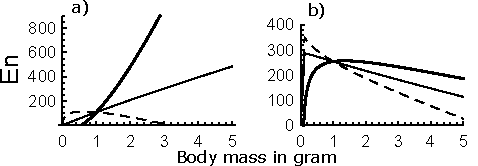
\includegraphics{Fig1}}
\caption{
	Duration of warm-up as a function of the timing of warm-up.
	Daily temperature varies from $15^{\circ}\rm{C}$ at sunrise and peaks at $30^{\circ}\rm{C}$ in the middle of the afternoon.
	Solar radiation is equivalent to what would happen at 30 degree latitude during to equinox clear sky.
	a) thickest, thick, thin, and dashed lines denote  $z = 10, 1, 0.1, 0.01$,  respectively.
	b)  Duration of warm-up with different conductance. Body size $z = 1$ , $a_w = 1.25$
	Default value for $K_1$ and $K_2$ .	
}% Add parameter values later
\label{fig5}
\end{center}
\end{figure}
\vspace{-1.5cm}
%%
\begin{figure}[H]
\begin{center}
%\scalebox{1.5}{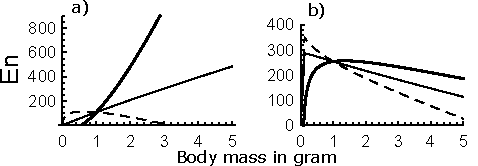
\includegraphics{Fig1}}
\caption{
	Shape of the fundamental niche as a function of temperature.
	a) As a function of when warm-up starts ($t_f = 1$ hour, early = sunrise, mid = sunrise+ 2 hr, late = sunrise + 4 hr, body size $z = 2$). 
	b) As a function of the exponent of $b_3$ ($t_f = 1$, large (black) = 2, small (gray) = 0.5).
	c)  As a function of resource availability. 
	Thick line = high resource (30), thin line = low resource (15).
	Thick and thin gray lines overlap because the small is not affected by resource loss. 
	  ($b_3 = b_2 = b_1 = 0.75$).
	Other parameters: $ b_2 = b_1  = 0.75,  a_2 = 10 a_1, a_w = 1.25$, and  $\rho = 30$.
}% Add non trivial units later
\label{fig6}
\end{center}
\end{figure}
%
%\begin{figure}[H]
%\begin{center}
%%\scalebox{1.5}{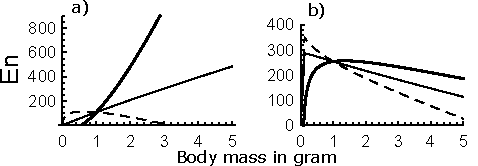
\includegraphics{Fig1}}
%\caption{
%	Shape of the fundamental niche as a function of temperature.
%	Except in d),  temperature is constant during the day.
%	a) The simplest case without warm-up, high resource availability (30 gram).
%	b) Halving resource availability and without warm-up.
%	c) Adding warm-up and  restoring resource availability to high, there is a penalty for long warm-up time as it reduces total foraging time, no change in temperature.
%	d) A complete  scenario with warm-up and variable temperature that increases from 15 to $30^{\circ} \rm{C}$ from sunrise to mid-afternoon.
%	Other parameters: $b_3 = 1, b_2 = b_1  = 0.75,  a_2 = 10 a_1, a_w = 1.25$, and  $\rho = 20$.
%}% Add non trivial units later
%\label{fig6}
%\end{center}
%\end{figure}
%

%\input{./Appendix_warm-up_derivation.tex }
\newpage

\bibliography{ref2}
\end{document}
